Resulting predictions are visually very similar to the ground truth fluorescence. The quality of the outputs are confirmed to be already good enough to enable wet lab scientists to advance the CLD process with the use of developed UNet model. Nevertheless, a more thorough visual evaluation of nuclei fluroescence predictions is provided in Figure \ref{fig:nuclei-troubles}. There are three main visible problems that should be addressed in further research:
\begin{itemize}
	\item The form of the nucleus is well-captured, but the texture inside is not (the change of intensities) is not predicted very well.
	\item The border around the nucleus is quite blurry.
	\item The overall intensities of predictions seem to be higher than the ground truth ones.
\end{itemize}

All of these problems are quite similar across other organelles predictions as well and can be summarized under the statement that the model does not have high enough resolution. Which can be solved by making a model larger and providing it with more data. In order to confirm this a bigger model has been trained.

Indeed, increasing the number of filters in each convolutional layer by a factor of $4$ (switching from from $16$ to $64$ in the first one) the model was able to capture more details. Predictions became better both visually (see Figure \ref{fig:better-nuclei}) and based on both metrics (PCC and MSE losses, see Figure \ref{fig:nuclei-comparison-predictions} "bigger model" bar (right)). For more details of the increased inference, training times and their costs refer to Appendix \ref{appendix:first}.

\begin{figure}[htb]
	\begin{center}
		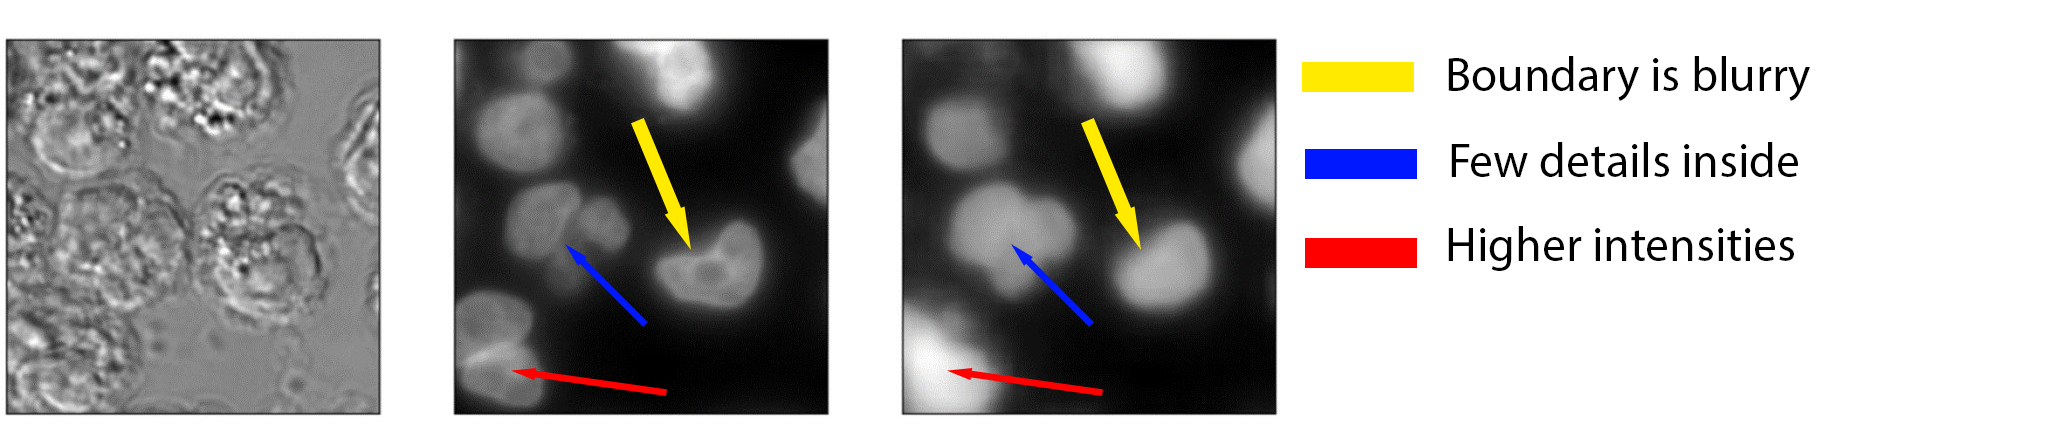
\includegraphics[width=\linewidth]{bilder/nuclei/problems.png}
		\caption[Typical challenges in predictions for nuclei in this study]%
		{Typical challenges in predictions for nuclei in this study. This figure depicts three main challenges in UNet predictions with nuclei target.}\label{fig:nuclei-troubles}
	\end{center}
\end{figure}

Another rather small issue is that predictions on the border of the crops seem to be worse than in the center. For example, see the cell located at the top left corner in Figure \ref{fig:nuclei-troubles} selected into a green circle. Nucleus of this cell is missing in the prediction image as the cell in not fully present in the DIC input. As already mentioned in section \ref{par:crops-combination}, when the cell is not fully present in the crop (split in halves, for example), the network does not have enough data to give out a good enough prediction. However, when combining crops into high-resolution images, this problem can be mitigated by the method described in section \ref{par:crops-combination}.

The problem of the higher intensities can also be addressed by a more careful dataset filtration, as several images with overexposed cells are still used for training. This might be a reason for the intensity of overprediction. Blurry borders are also a signal indicating an overexposed nucleus. Even if they are present in the dataset, they can be removed using background removal techniques described in Section \ref{section:background-removal}. This was not done in the scope of this research as the predictions have had good enough quality to be used in the CLD process.

\begin{figure}[htb]
	\begin{center}
		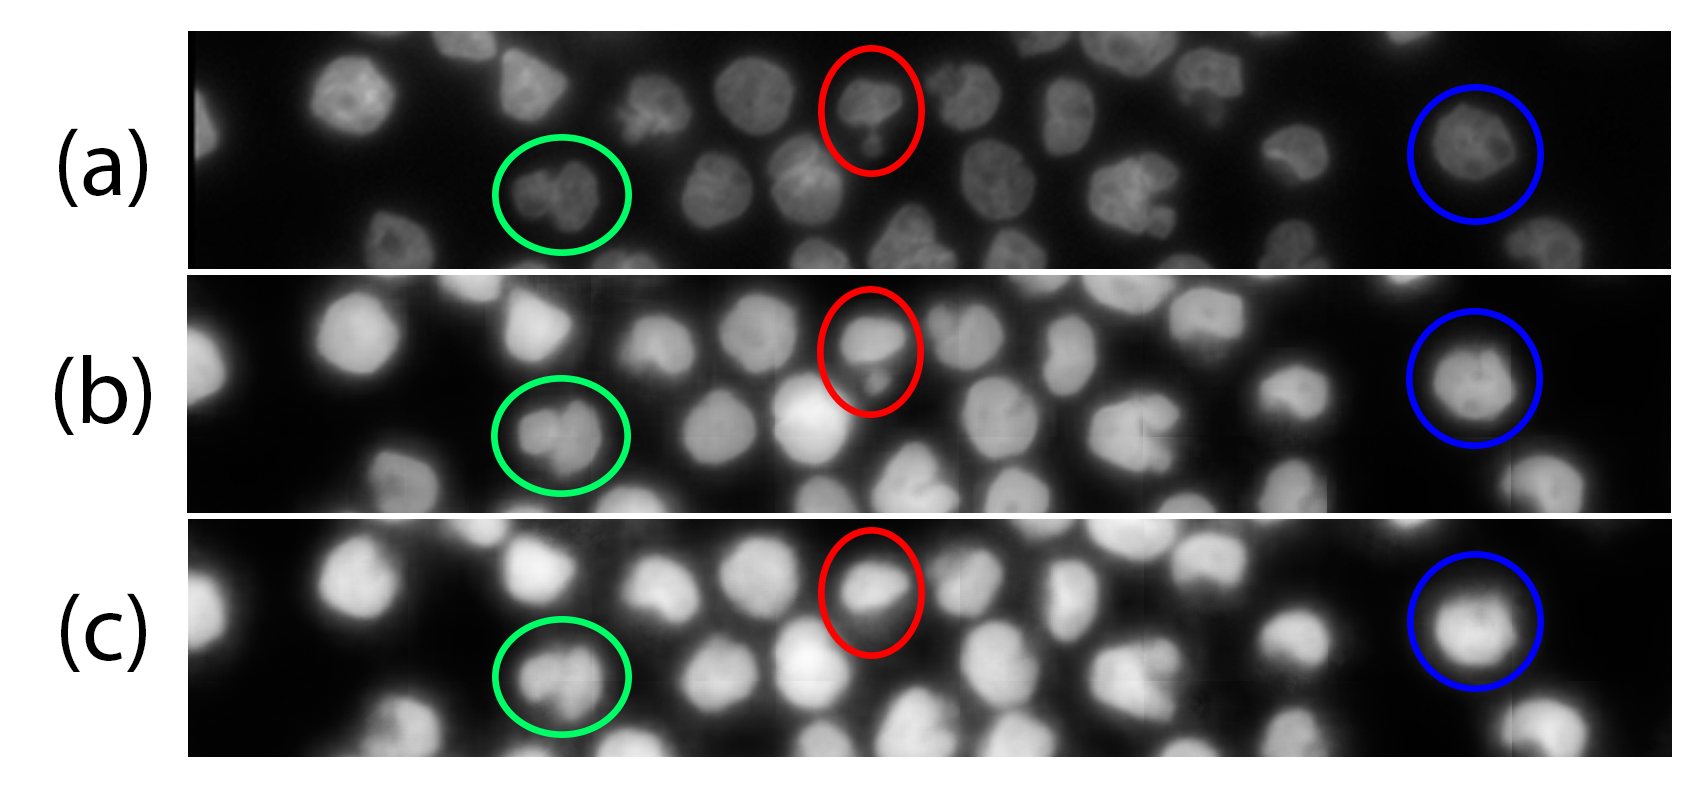
\includegraphics[width=0.6\linewidth]{bilder/nuclei/bigger-model.png}
		\caption[Predictions improvement]%
		{Predictions improvement: (a) ground truth fluorescence; (b) bigger model with four times more filters in convolutional layers; (c) standard architecture. Image resolution (amount of details captured) is clearly better for a UNet of a bigger size (b). }\label{fig:better-nuclei}
	\end{center}
\end{figure}
